
%(BEGIN_QUESTION)
% Copyright 2015, Tony R. Kuphaldt, released under the Creative Commons Attribution License (v 1.0)
% This means you may do almost anything with this work of mine, so long as you give me proper credit

\noindent

\vskip 5pt

\vskip 5pt
\begin{center}
\textbf{Målesystemer -- Nivå 1 }
\vskip 5pt 
\textbf{Arbidsoppdrag på Stasjon 9}
\vskip 5pt 
\textbf{Oppsett av målesystemer for nivå}
\end{center}

\textbf{Introduksjon}

I dette arbeidsoppdraget skal du jobbe med målesystemer for nivå. Du skal utføre sjekk og kalibrering for nivåmålesystemer basert på følgende prinsipper:
\begin{itemize}[noitemsep]
	\item Ultralyd
	\item Trykk
	\item Radar
\end{itemize}
Du skal sette i stand målesystemene for nivå på de tre tankene på denne stasjonen. Alt må koblet opp og virke mot stasjonens styresystem. 
$$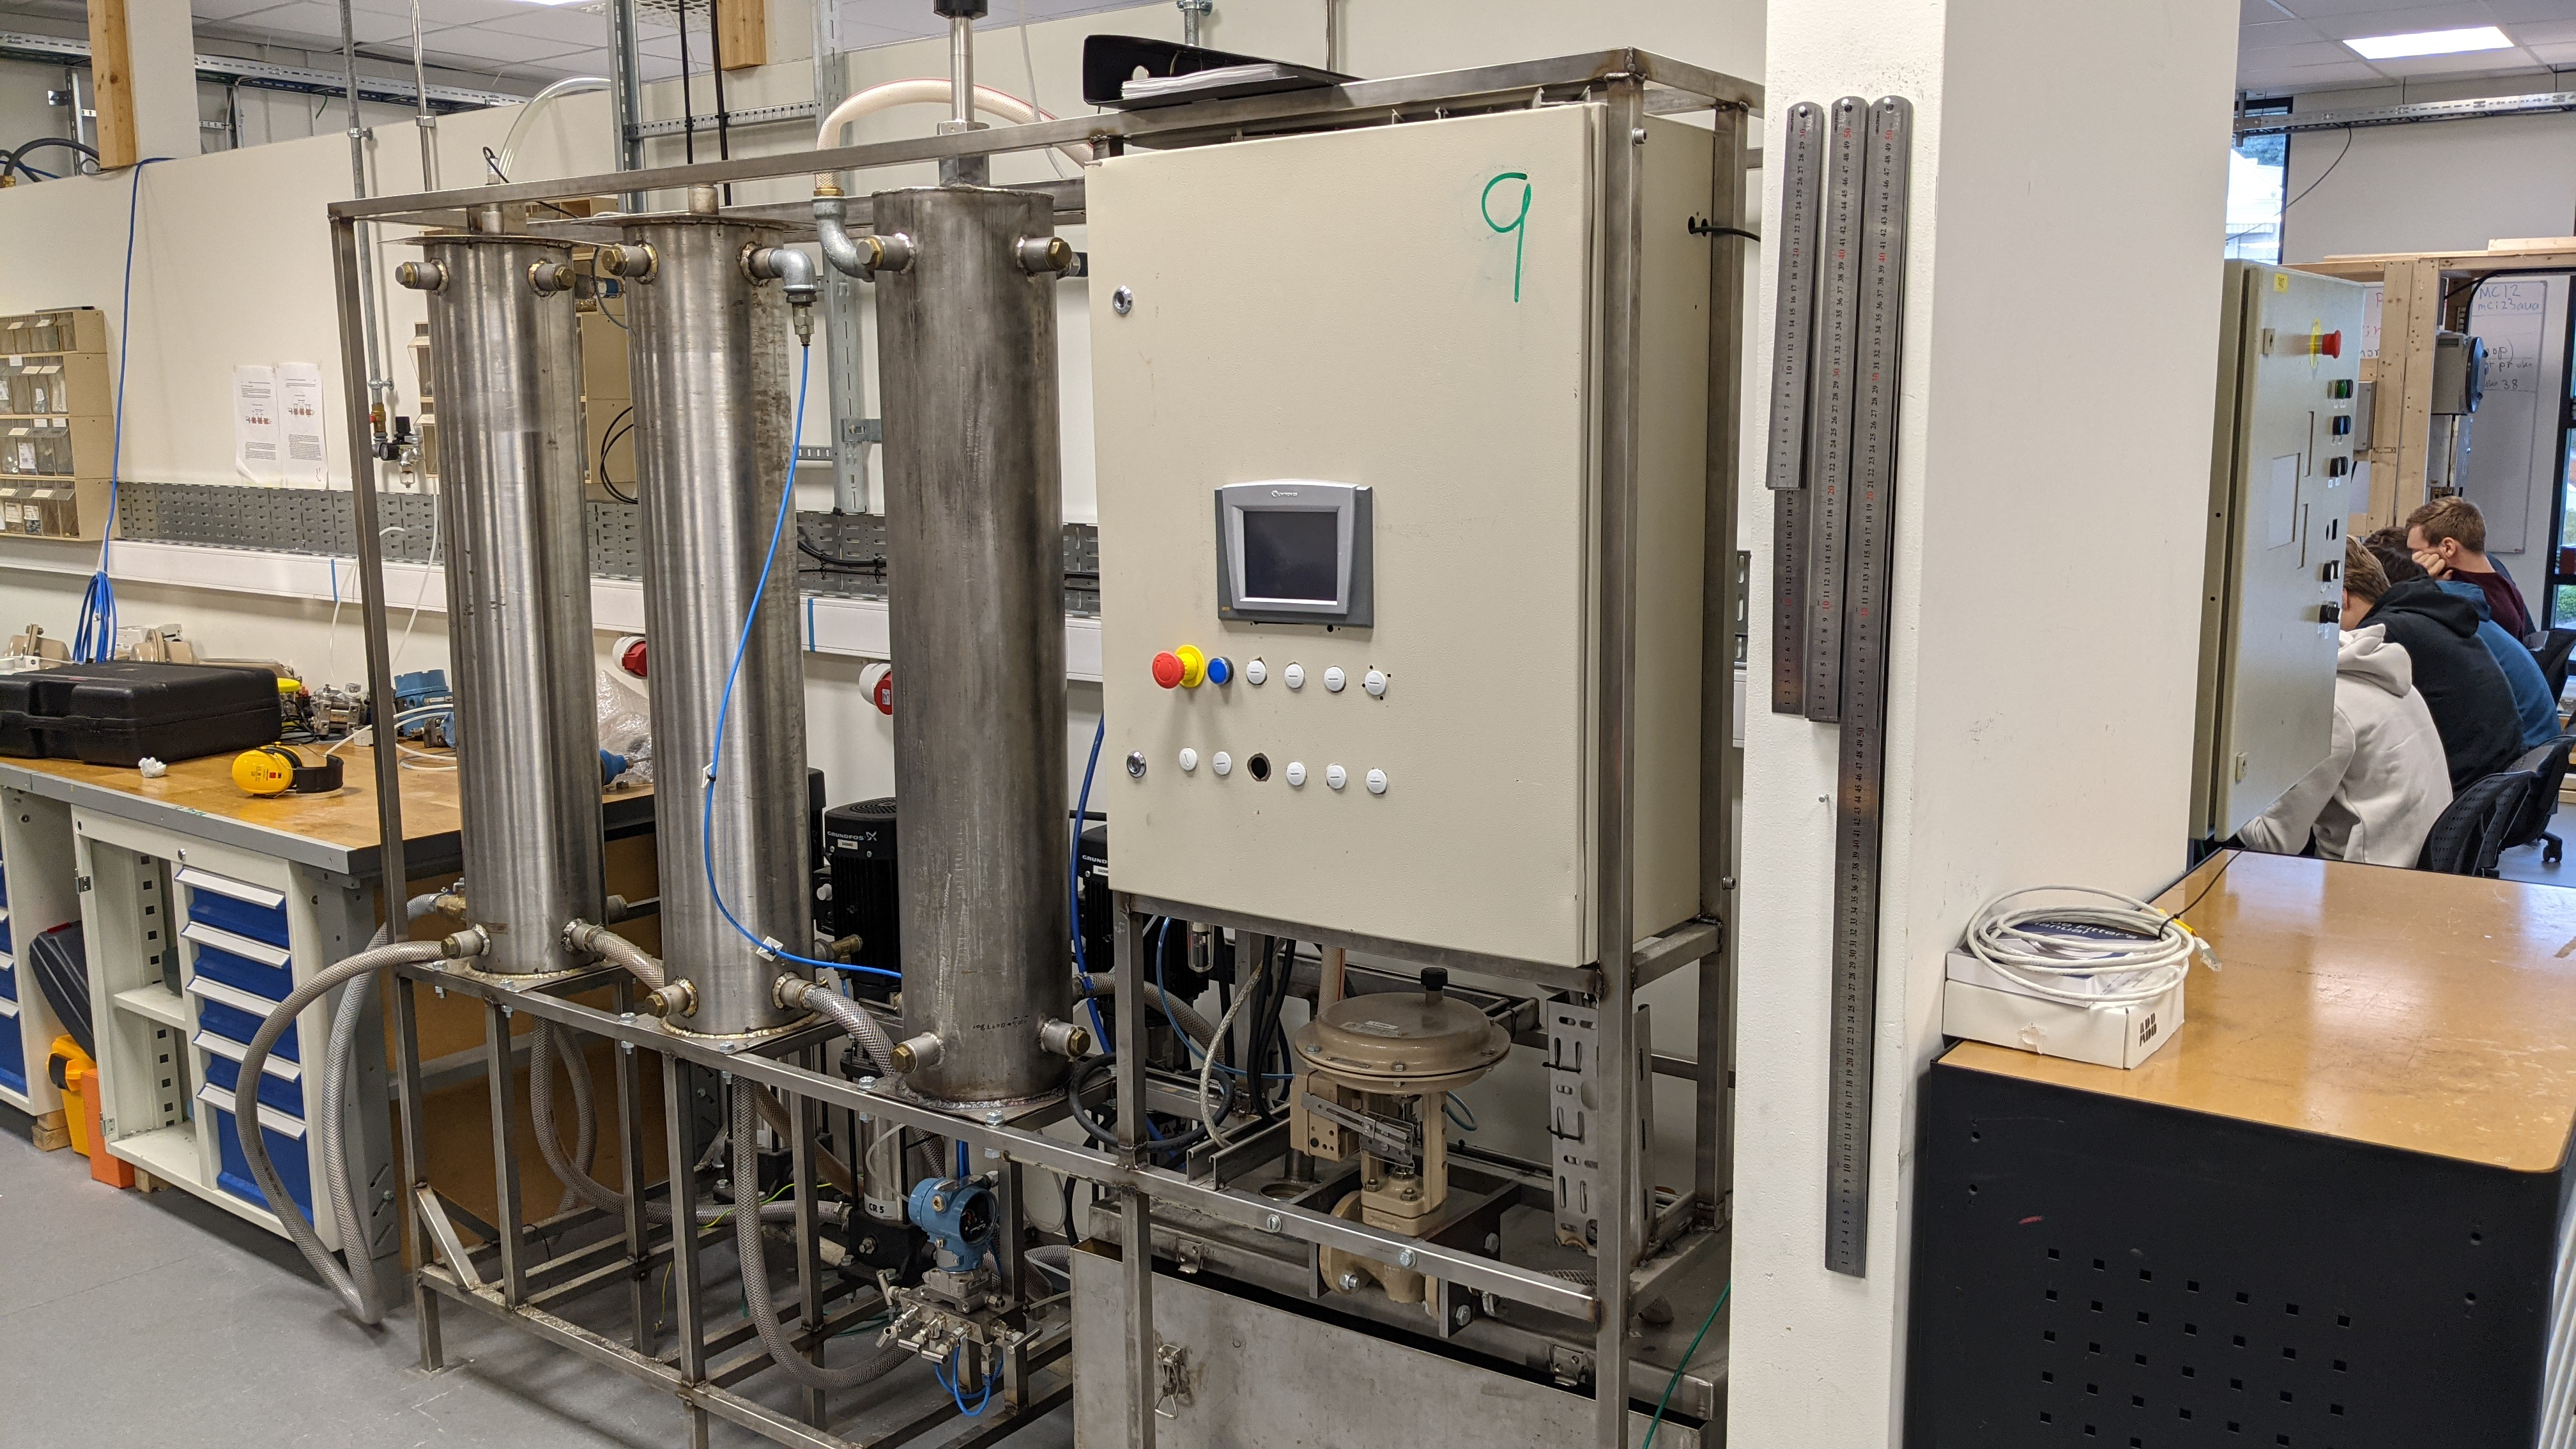
\includegraphics[width=10.5cm]{stasjon09x01.jpg}$$
\textbf{Kalibrering og justering range for en smart transmitter}
Målet med oppgaven er å lære hvordan vi justerer en transmitter for trykk.


\vskip 5pt 

\textbf{Teorioppgaver}
\vskip 5pt 
\href {https://autofaget.no/level/node2.html} {Leseoppgave}
\vskip 5pt 
\textbf{Planlegging}
\vskip 5pt 


\textbf{Gjennomføring}
\vskip 5pt 

\textbf{Dokumentasjon}
\vskip 5pt 

\begin{enumerate}
	\item Beskriv hvordan du planla, gjennomførte og dokumentere jobben. Forklar eventuelle avvik dere måtte observere under oppdraget. 
	\item Dokumentasjonen skal inneholde sløyfeskjema av alle sløyfer du har jobbet med. 
	\item Kalibreringsskjema for alle sløyfene
	\item Bilder av transmittere
\end{enumerate}










\vfil 


\underbar{file i04843}
\vfil \eject
%(END_QUESTION)





%(BEGIN_ANSWER)


%(END_ANSWER)





%(BEGIN_NOTES)


%INDEX% Arbeisdoppdrag, Målesystemer, Nivå 1, Stasjon10, Kalibrering, DP-celle(Smart)

%(END_NOTES)


